\documentclass{beamer}
\usepackage{graphicx}
\usepackage{epstopdf}
\usepackage{hyperref}
\usecolortheme{seagull}

\title{USRP based Cognitive Radio Test-bed using OpenBTS}
\author{Abrar Ahmad (113310017) \\ Swrangsar Basumatary (09d07040) }
\institute{Department of Electrical Engineering \\ IIT Bombay, Powai}
\date{June 2014}

\setbeamertemplate{frametitle}[default][center]
    
\begin{document}
  \frame{\titlepage}


	\begin{frame}{Problem Statement}
    	\begin{itemize}
    		\item To develop a testbed for cognitive radio demonstrating coexistence of primary (licensed) users and secondary (unlicensed users)
    		\item A two frequency testbed (channels used 945 MHz and 955 MHz)
    		\item A four frequency testbed (936 MHz, 943 MHz, 950 MHz, 957 MHz)
    	\end{itemize}
	\end{frame}
	
	\begin{frame}{Overview of the tasks accomplished in our project}
		\begin{itemize}
      \item Cognitive radio?,  spectrum holes?
      \item GNURadio
      \item Python programming language
      \item USRP kit
      \item OpenBTS
      \item Calls and SMS service on local network
      \item Spectrum sensing techniques
      \item Defining problem statement
    \end{itemize}
  \end{frame}
    
    \begin{frame}{}
        \begin{itemize}
		\item Developing a flow chart of the solution to this problem
		\item Running GNURadio and OpenBTS  on the same computer at the same time
		\item Bash scripting ( .sh files)
		\item Periodogram analysis
		\item Building a two frequency cognitive radio test bed
		\item Building a four frequency cognitive radio test bed
		\end{itemize}
	\end{frame}
	
	\begin{frame}{Hardware and software used}
    \begin{itemize}
      \item GNURadio
      \item OpenBTS
      \item USRP N210  Kits
      \item GSM mobile phones with SIM cards
      \item Computers
    \end{itemize}
  \end{frame}

  \begin{frame}{Setup for the two-frequency testbed}
    \begin{figure}
      \centering
      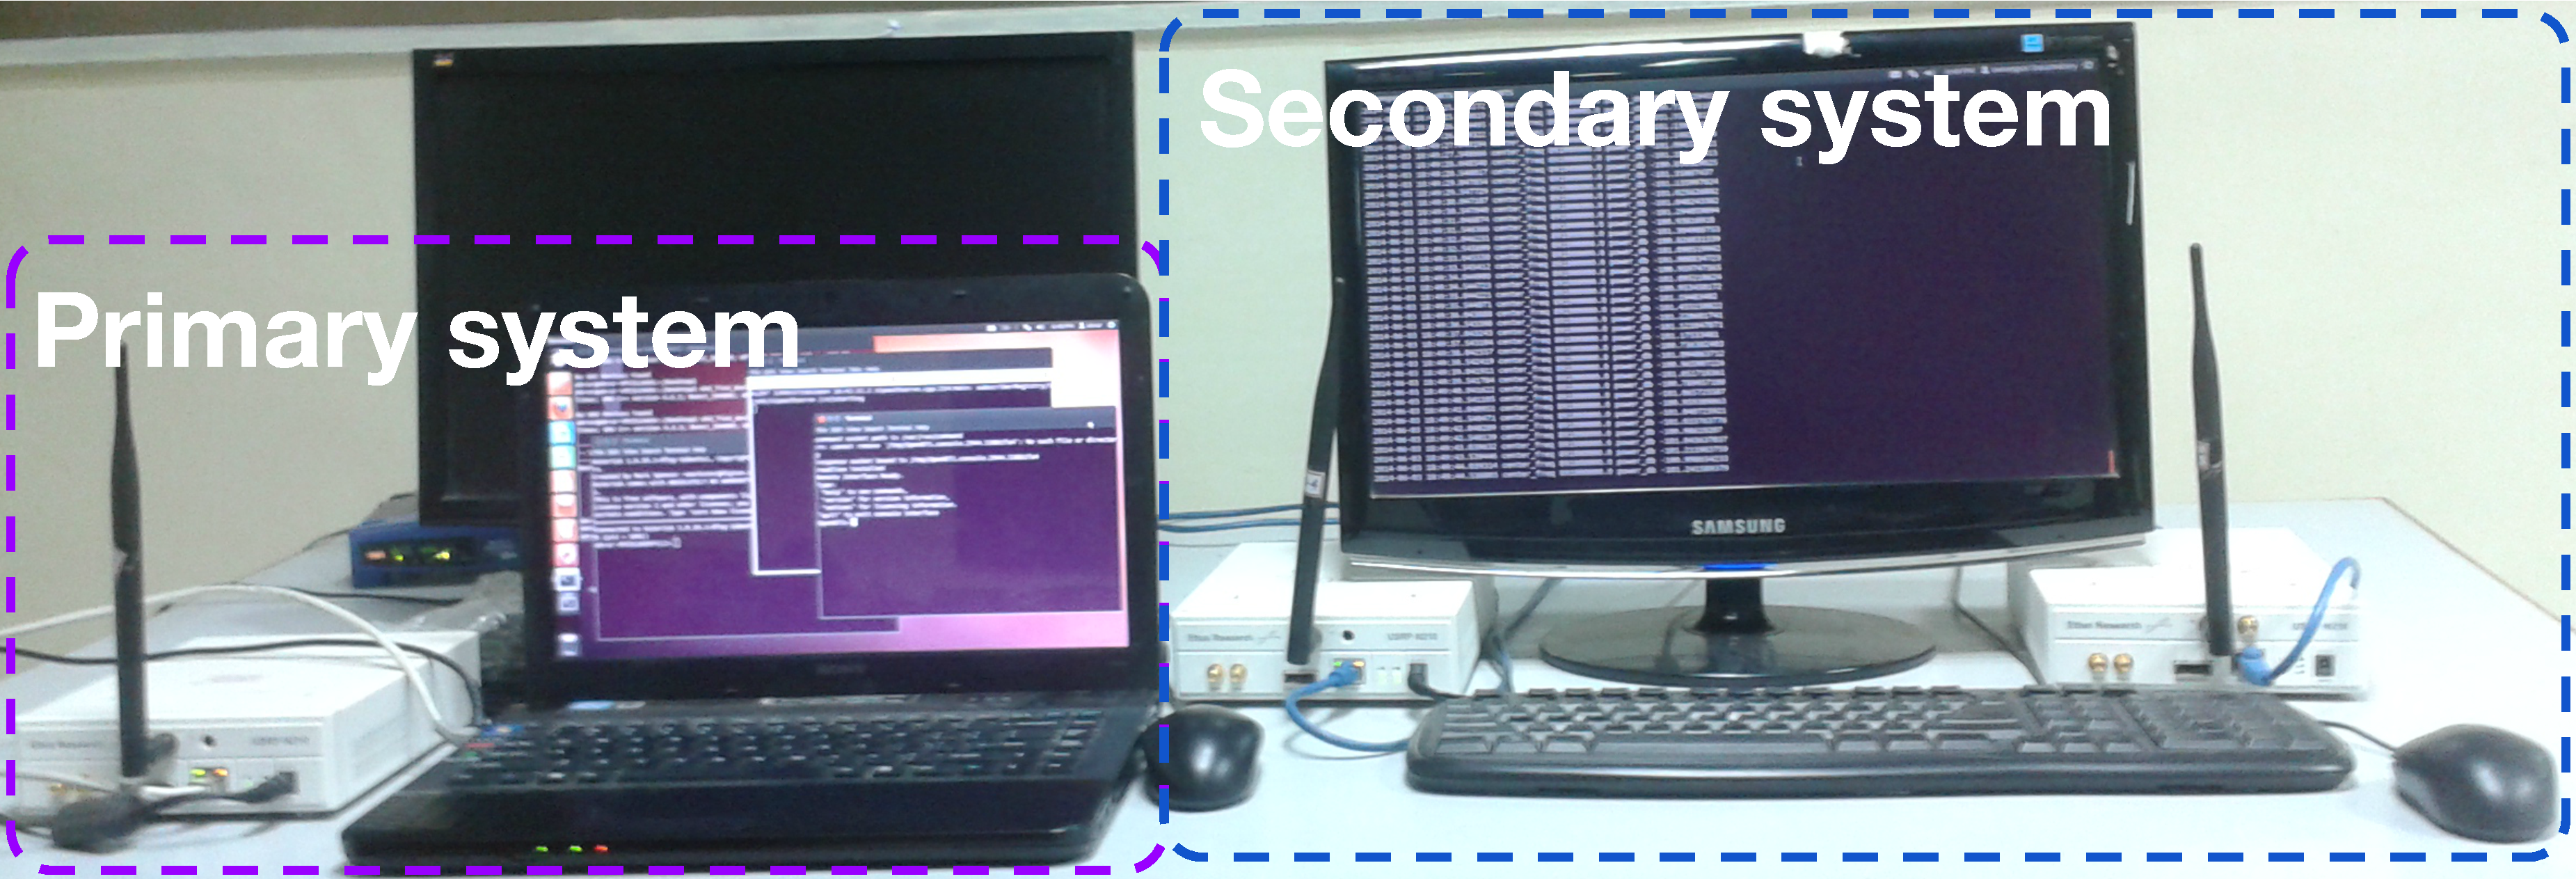
\includegraphics[width=\linewidth]{img/freq2}
    \end{figure}
  \end{frame}
  
  \begin{frame}{Setup for the four-frequency testbed}
    \begin{figure}
      \centering
      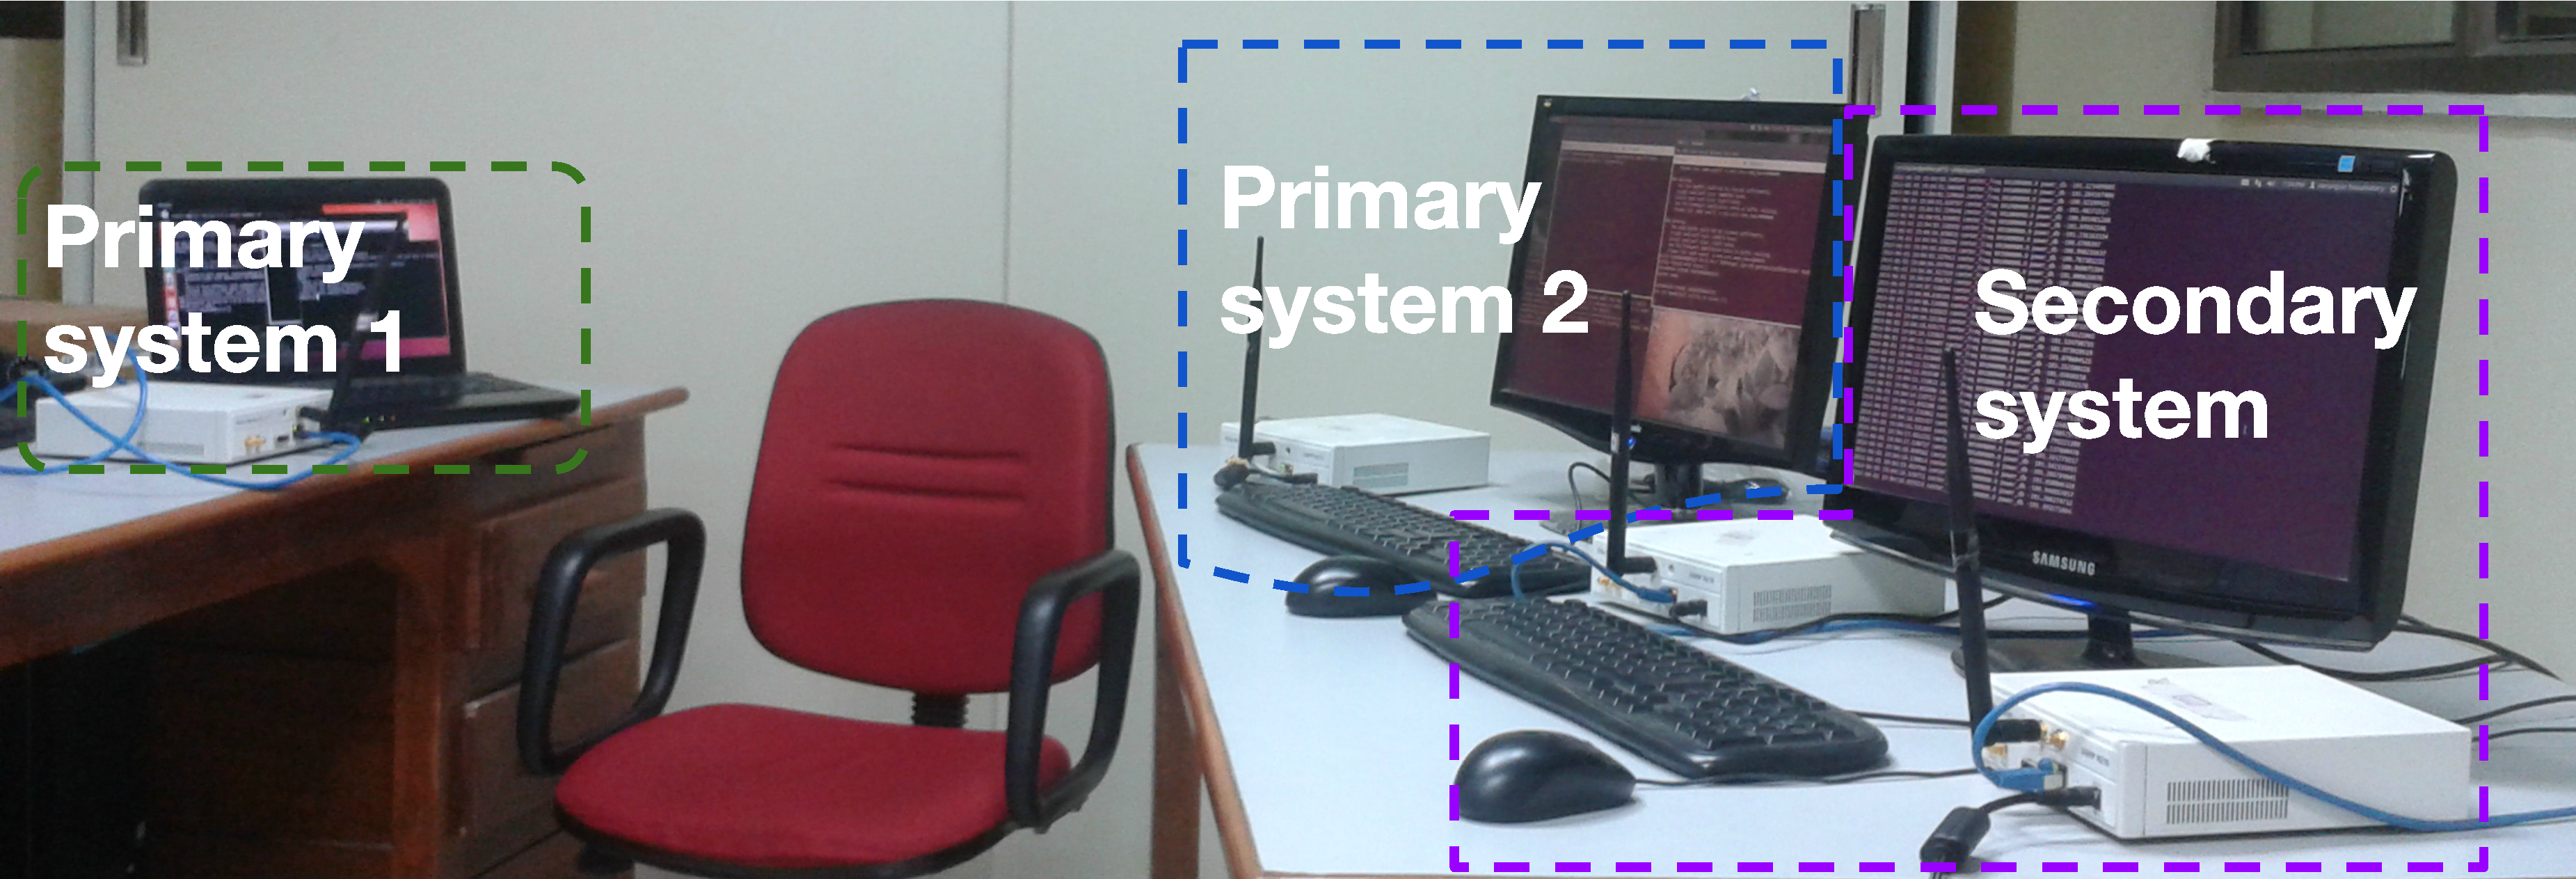
\includegraphics[width=\linewidth]{img/freq4}
    \end{figure}
  \end{frame}
    
  \begin{frame}{Cognitive Radio}
    \begin{minipage}[t][0.8\textheight][t]{\textwidth}
      \begin{itemize}
        \item What is Cognitive Radio?
      \end{itemize}
      \begin{figure}
        \centering
        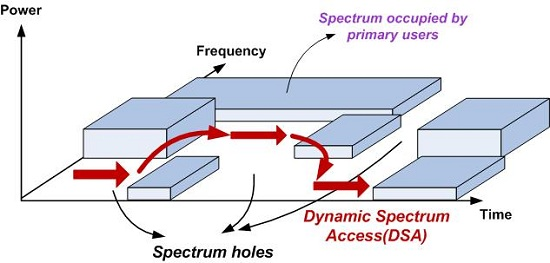
\includegraphics[width=0.8\linewidth]{img/freqUtil}
      \end{figure}
      \vfill
      \tiny{Source: \url{http://www.brunel.ac.uk/\_\_data/assets/image/0011/237539/Abdullah-Masrub1.jpg}}
    \end{minipage}
  \end{frame}


    
\end{document}